\section{انواع تجزیه}
\begin{frame}[standout]
تجزیه CP
\end{frame}
\begin{frame}
تجزیه CP یک تانسور، مجموع اجزای رتبه یک تانسور است. به عنوان مثال؛ تانسور سه بعدی 
$\mathcal{X}\in \mathbb{R}^{I\times J\times K}$
را می‌توانیم به صورت زیر تقریب بزنیم.
\[\mathcal{X}\approx \sum_{r=1}^Ra_r \circ b_r \circ c_r,\]
که در آن $R$ یک عدد مثبت و  
$a_r\in\mathbb{R}^I$،
$b_r\in\mathbb{R}^J$
و
$c_r\in\mathbb{R}^K$
است.

\pause
\begin{center}
	\includegraphics[width=0.8\textwidth]{img/ok/cp.pdf}
\end{center}
\end{frame}

\begin{frame}
\small{
فرض کنید که هدف محاسبه بهترین تقریب برای تانسور سه بعدی 
$\mathcal{X}$
است. 

\begin{align*}
\min\limits_{\hat{\mathcal{X}}}\|\mathcal{X}-\hat{\mathcal{X}}\|
\quad \text{با}\quad
\hat{\mathcal{X}}=\sum_{r=1}^R \lambda_r a_r\circ b_r\circ c_r=[\lambda;A,B,C].
\end{align*}
که می‌توان با ثابت فرض کردن $A$ و $B$، 
برای $A$ حل کرد و همینطور به صورت تکراری برای ماتریس‌های دیگر.
}
\end{frame}
\begin{frame}[standout]
HOSVD
\end{frame}
\begin{frame}{HOSVD}
\begin{center}
	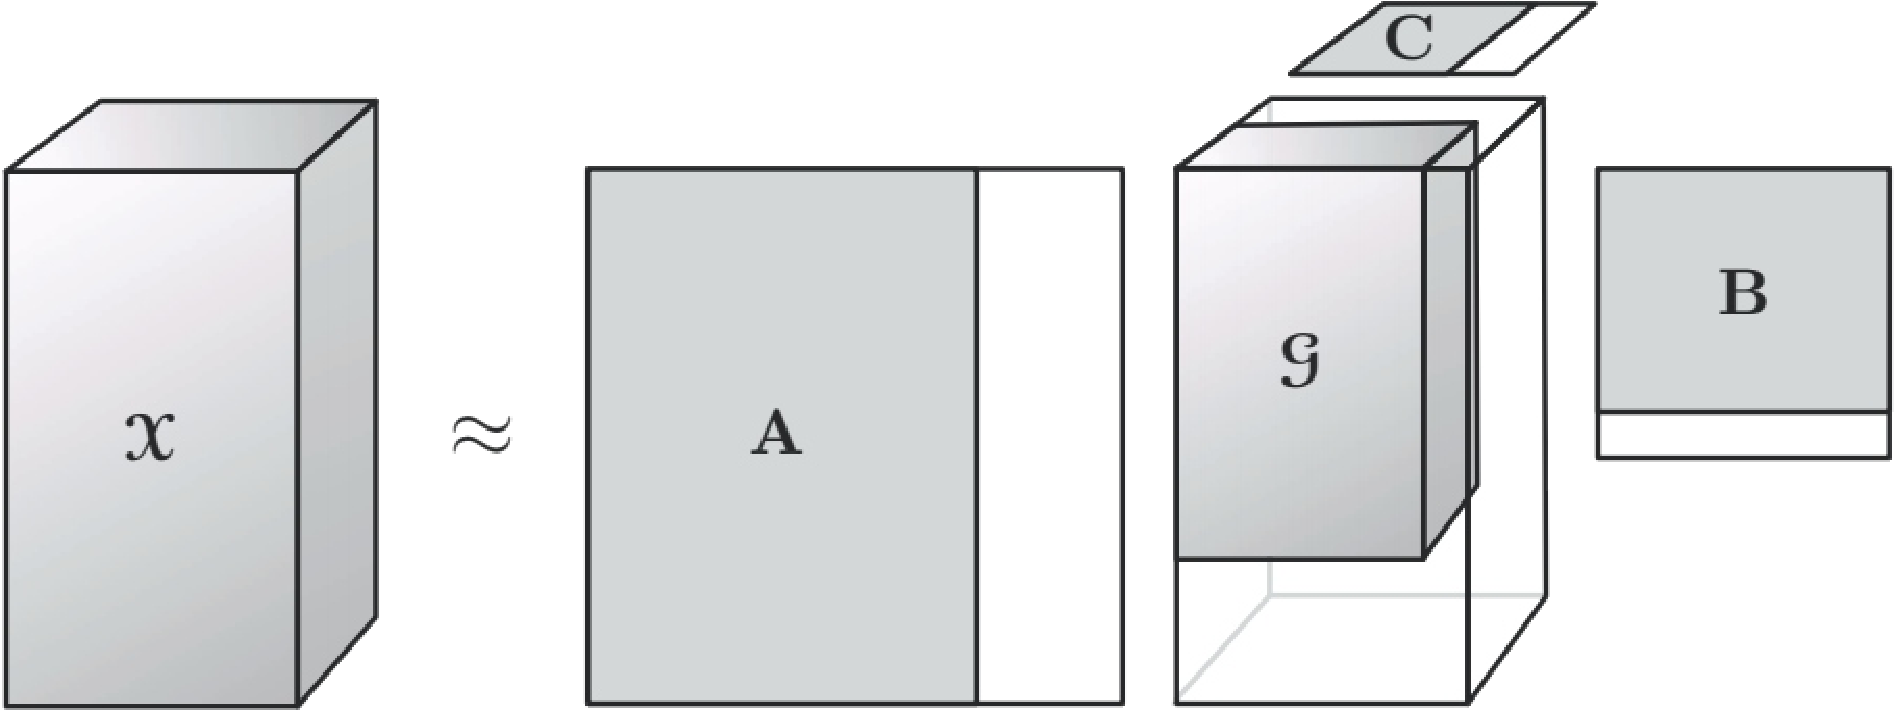
\includegraphics[width=1\textwidth]{img/ok/HOSVD.pdf}
\end{center}
\begin{center}
	تجزیه
	HOSVD
\end{center}
\end{frame}
\begin{frame}{HOSVD}
\begin{center}
	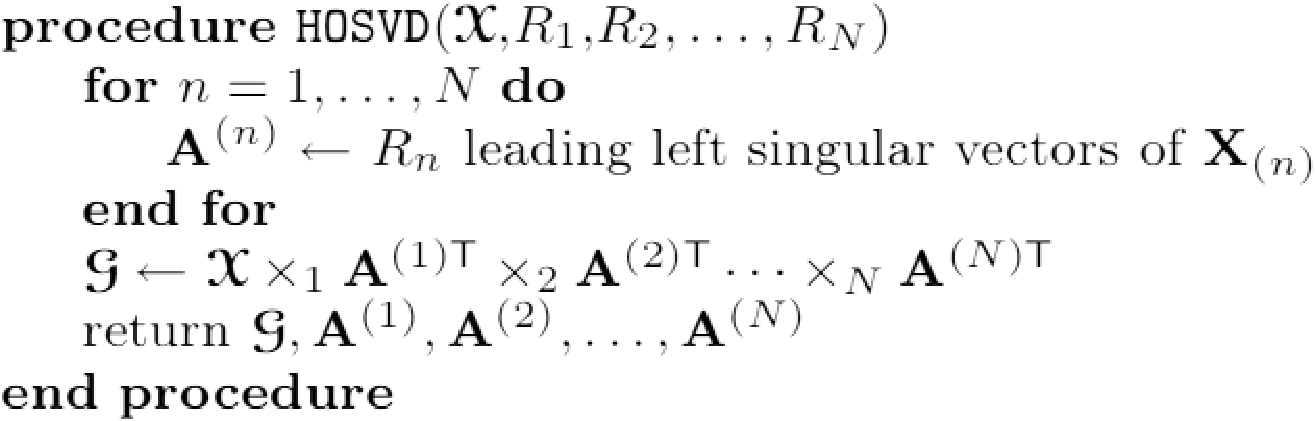
\includegraphics[width=0.7\textwidth]{img/ok/alHOSVD.pdf}
\end{center}
\pause
\small{
هدف محاسبه مسئله بهینه سازی زیر است:
\begin{align*}
&\min\limits_{\mathcal{G},A^{(1)},\cdots,A^{(N)}} \|\mathcal{X}-[\mathcal{G};A^{(1)},\cdots,A^{(N)}]\|\\
&s.t \qquad \mathcal{G}\in\mathbb{R}^{R_1\times \cdots\times R_N}
\end{align*}
که در آن
$A^{(n)}\in\mathbb{R}^{I_n\times R_n}$
و متعامد است.
}
\end{frame}